\chapter{SLAM}

\paragraph*{}
In the previous semester, we selected GRAPH SLAM as our preferred SLAM approach. Initially, we planned to implement GRAPH SLAM within Webots using a GitHub package by Hobby Singh called Graph-SLAM. We specifically utilized the 2D LiDAR module, as our project solely relies on a 2D LiDAR without any camera input. However, we encountered challenges with this implementation because the package required a dataset composed of .clf files containing odometry and LiDAR logs. Although we successfully extracted the necessary logs, we continuously encountered an ICP error, suggesting that our dataset might have been missing certain fields or that the SLAM package needed fine-tuning for our specific project requirements. While the generated map accurately reflected the odometry poses and edges, the LiDAR readings resulted in unclear, hazy lines. After multiple attempts to resolve these issues, we decided to develop our own version of Graph SLAM while temporarily switching to the ROS2 SLAM package known as SLAM Toolbox.

\begin{figure} [H]
    \centering
    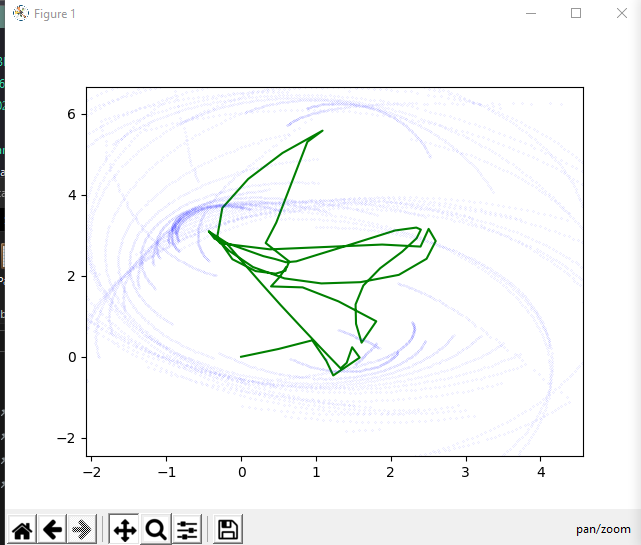
\includegraphics[width=0.5\linewidth]{assets/images/slam/graph_slam.png}
    \caption{Map generated from the GRAPH SLAM package}
    \label{fig:graph_slam_map}
\end{figure}

\paragraph*{}
SLAM Toolbox is essentially a graph-based SLAM solution that utilizes pose graph optimization to refine map accuracy and correct errors in localization. It represents robot poses as nodes and constraints (such as odometry and scan matching) as edges, forming a graph structure that can be optimized to minimize drift and inconsistencies. This graph-based approach allows for efficient loop closure detection, ensuring that previously visited areas are correctly aligned, even in large or dynamic environments. By leveraging modern optimization techniques like Ceres Solver, SLAM Toolbox continuously refines the pose graph, making it a powerful and flexible tool for real-time mapping and localization in ROS2-based robotic applications. We initially tested SLAM Toolbox in a Gazebo simulation, where we successfully generated an accurate map. However, since this was purely in a simulated environment, transitioning to real-world implementation requires actual odometry data for accurate mapping and localization.

\begin{figure} [H]
    \centering
    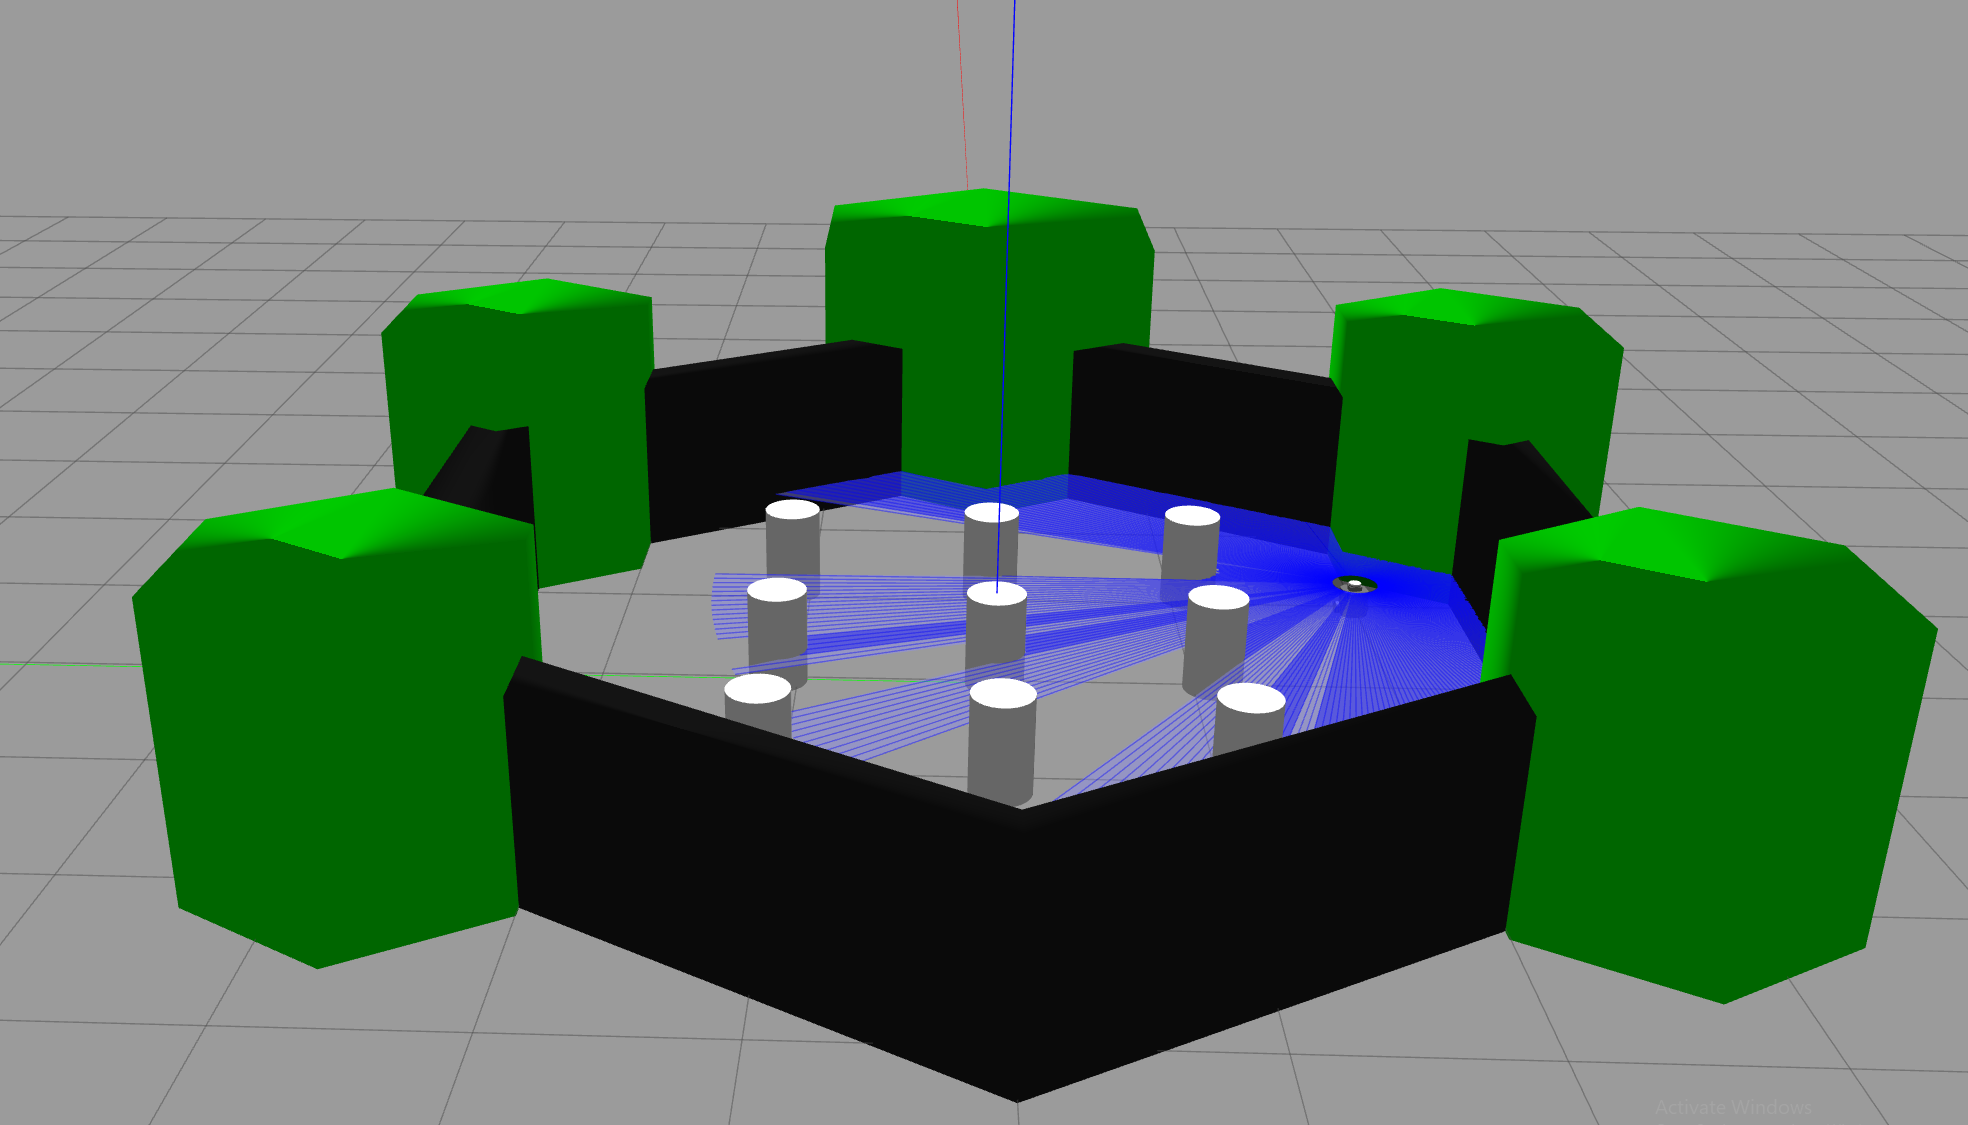
\includegraphics[width=0.5\linewidth]{assets/images/slam/gazebo_test_world.png}
    \caption{The Gazebo world}
    \label{fig:gazebo_map}
\end{figure}

\begin{figure} [H]
    \centering
    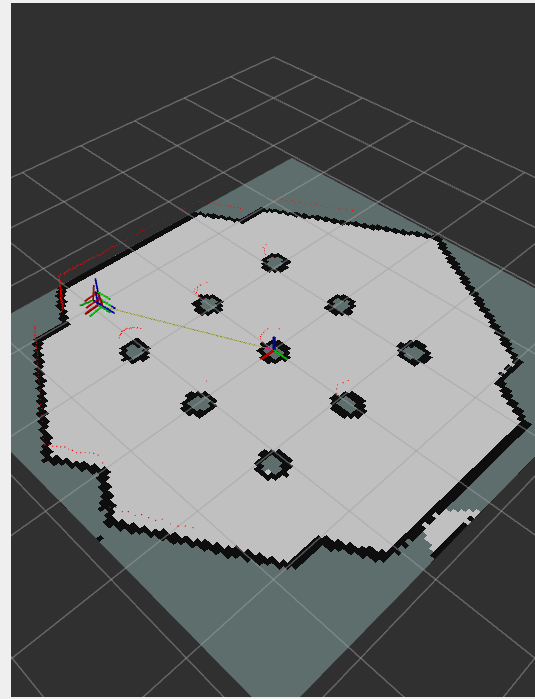
\includegraphics[width=0.5\linewidth]{assets/images/slam/slam_toolbox.png}
    \caption{Map generated from SLAM Toolbox}
    \label{fig:graph_slam_map}
\end{figure}

